\documentclass[a4paper, 12pt, oneside]{scrbook}

\input{settings.tex}

\bibliography{bibliography.bib}
\begin{document}

\frontmatter

% Hierin müssen Matrikelnummer Name usw. gesetzt werden.

\input{prefix/title.tex}

\pagenumbering{gobble}
\input{prefix/eigenstaendigkeit.tex}
\section*{Kurzzusammenfassung}

Diese Studienarbeit behandelt die Entwicklung einer webbasierten Todo-Liste mit Vue.js, Spring Boot und MySQL mit Test-Driven Development. Ziel ist es, eine effiziente Aufgabenverwaltung zu ermöglichen, inklusive Erstellung, Bearbeitung und Löschung von Todos.

Die Arbeit beschreibt detailliert die Architektur, Implementierung und Teststrategie der Anwendung. Trotz grundlegender Funktionen wie Benutzerregistrierung und -anmeldung fehlen sichere Abmeldung und Todo-Bearbeitung, was Privatsphäre und Benutzerfreundlichkeit beeinträchtigt.

Ursachen sind mangelnde Erfahrung des Entwicklers, schlechtes Zeitmanagement und unvollständige TDD-Anwendung, was zu fehlerhaftem Code führte. Die Arbeit bietet Einblicke und Empfehlungen für zukünftige Verbesserungen und eine stärkere Anwendung bewährter Methoden.

\section*{Abstract}

This student research project deals with the development of a web-based todo list using Vue.js, Spring Boot and MySQL with Test-Driven Development. The aim is to enable efficient task management, including the creation, editing and deletion of todos.

The work describes in detail the architecture, implementation and test strategy of the application. Despite basic functions such as user registration and login, secure logout and todo editing are missing, which impairs privacy and user-friendliness.

Causes include lack of developer experience, poor time management and incomplete TDD application, resulting in buggy code. The work provides insights and recommendations for future improvements and greater use of best practices.






\tableofcontents

% Abbildungsverzeichnis
\cleardoublepage
\phantomsection
\addcontentsline{toc}{chapter}{\listfigurename}
\pagenumbering{Roman}
\listoffigures

% Tabellenverzeichnis
% \cleardoublepage
% \phantomsection
% \addcontentsline{toc}{chapter}{\listtablename}
% \listoftables

%Codebeispiel Verzeichnis
% \cleardoublepage
% \phantomsection
% \addcontentsline{toc}{chapter}{\lstlistlistingname}
% \lstlistoflistings

% Abkürzungsverzeichnis (siehe Ordner "prefix")
\input{prefix/abbreviation.tex}

\mainmatter

% Inhalt (siehe Ordner "content") %
\chapter{Einleitung}

Die Notwendigkeit effektiver Aufgabenverwaltungslösungen ist in unserer zunehmend digitalisierten Welt unbestreitbar. Eine Todo-Liste ist ein bewährtes Werkzeug, das Einzelpersonen und Teams hilft, ihre täglichen Aufgaben zu organisieren, zu priorisieren und zu verfolgen. In einer Zeit, in der Effizienz und Produktivität entscheidend sind, bietet eine gut gestaltete Todo-Liste klare Vorteile bei der Strukturierung des Arbeitsalltags.

Ziel dieser Studienarbeit ist es, eine webbasierte Todo-Liste mit Test-Driven Development zu entwickeln, die Benutzern eine intuitive und effiziente Möglichkeit bietet, ihre Aufgaben zu verwalten. Die Anwendung soll es Einzelpersonen ermöglichen, Todos zu erstellen, zu bearbeiten und zu löschen und die Möglichkeit bieten eine Beschreibung, ein Fälligkeitsdaten, sowie das Markieren des Erledigen einer Todo hinzuzufügen. Darüber hinaus soll die Todo-Liste Funktionen wie Benutzerregistrierung und -authentifizierung bereitstellen, um die Sicherheit und Privatsphäre der Benutzerdaten zu gewährleisten.

Im Rahmen dieser Entwicklung werden zwei Hauptkomponenten erstellt: das Frontend, das die Benutzeroberfläche der Todo-Liste bereitstellt, und das Backend, das die Datenverarbeitung und -speicherung übernimmt. Die Anwendung wird auf modernen Technologien basieren, darunter Vue.js für das Frontend, Spring Boot für das Backend, MySQL als relationale Datenbank.


Es werden grundlegende Kenntnisse in HTML, CSS, JavaScript, sowie in der Entwicklung mit Vue.js, Spring Boot, MySQL vorausgesetzt.

Diese Dokumentation bietet einen umfassenden Einblick in die Architektur, Implementierung und Teststrategie der Todo-Liste Webanwendung.
\input{content/grundlagen.tex}
\chapter{Konzeption und Design der Todo-App}
\section{Architektur der Anwendung}
Die Todo-App ist als eine mehrschichtige Architektur konzipiert, die eine klare Trennung der Verantwortlichkeiten zwischen den verschiedenen Schichten sicherstellt. Diese Architektur umfasst die folgenden Schichten:

\begin{itemize}
	\item \textbf{Präsentationsschicht}: Diese Schicht besteht aus REST-Controllern, die HTTP-Anfragen entgegennehmen und HTTP-Antworten zurückgeben. Sie interagiert mit der Service-Schicht, um Geschäftslogik zu implementieren.
	\item \textbf{Service-Schicht}: Diese Schicht enthält die Geschäftslogik der Anwendung. Sie validiert die Daten und ruft die entsprechenden Methoden der Repository-Schicht auf.
	\item \textbf{Repository-Schicht}: Diese Schicht besteht aus JPA-Repositories, die für die Datenzugriffslogik verantwortlich sind. Sie interagiert mit der MySQL-Datenbank, um Daten zu speichern und abzurufen.
	\item \textbf{Sicherheitsschicht}: Diese Schicht nutzt Spring Security, um Authentifizierung und Autorisierung zu implementieren. JWT (JSON Web Tokens) wird verwendet, um die Benutzersitzungen zu verwalten.
	\item \textbf{Datenbank-Schicht}: Diese Schicht besteht aus einer MySQL-Datenbank, in der alle Daten der Anwendung gespeichert werden.
\end{itemize}

\section{Datenmodell und Datenbankdesign}

\subsection{Entwurf des Datenmodells}
Das Datenmodell der Todo-App umfasst mehrere Entitäten, um die Beziehungen zwischen Benutzern und ihren Aufgaben zu verwalten. Die Hauptentitäten sind User und Todo.

\textbf{User Entität}

Die User-Entität repräsentiert einen Benutzer der Anwendung und enthält folgende Attribute:

\begin{itemize}
	\item id: Ein eindeutiger Bezeichner für jeden Benutzer.
	\item username: Der Benutzername, den der Benutzer zur Anmeldung verwendet.
	\item password: Das verschlüsselte Passwort des Benutzers.
\end{itemize}

Die User-Entität wird als Java-Klasse implementiert und mit JPA-Anmerkungen versehen, um die Zuordnung zur Datenbank zu erleichtern.

\begin{lstlisting}
	@Entity
	public class User {
		
		@Id
		@GeneratedValue(strategy = GenerationType.IDENTITY)
		private Long id;
		
		@Column(unique = true, nullable = false)
		private String username;
		
		@Column(nullable = false)
		private String password;
		
		// Getter und Setter
	}
\end{lstlisting}
	
\textbf{Todo Entität}

Die Todo-Entität repräsentiert eine Aufgabe und enthält folgende Attribute:

\begin{itemize}
	\item id: Ein eindeutiger Bezeichner für jede Todo.
	\item title:  Der Titel der Todo.
	\item description: Eine Beschreibung der Todo.
	\item dueDate: Das Fälligkeitsdatum der Todo.
	\item completed: Ein boolescher Wert, der angibt, ob die Todo abgeschlossen ist.
	\item user: Eine Beziehung zum Benutzer, der die Todo erstellt hat.
\end{itemize}

Die Todo-Entität wird als Java-Klasse implementiert und mit JPA-Anmerkungen versehen, um die Zuordnung zur Datenbank zu erleichtern.

\begin{lstlisting}
	@Entity
	public class Todo {
		
		@Id
		@GeneratedValue(strategy = GenerationType.IDENTITY)
		private Long id;
		
		@Column(nullable = false)
		private String title;
		
		@Column
		private String description;
		
		@Column
		private LocalDate dueDate;
		
		@Column(nullable = false)
		private boolean completed;
		
		@ManyToOne
		@JoinColumn(name = "user_id", nullable = false)
		private User user;
		
		// Getter und Setter
	}
\end{lstlisting}

\subsection{Projektanforderungen an die Datenbank}

Das Projekt stellt spezifische Anforderungen an die Datenbank, die durch MySQL erfüllt werden:

\begin{itemize}
	
	\item \textbf{Open source}: Die Datenbank muss open source sein, da keine Kosten für die Verwendung der Datenbank anfallen dürfen. My SQL bietet eine MySQL Community Edition an, die open source ist \cite{noauthor_mysql_nodate}.
	\item \textbf{Datenintegrität und Konsistenz}: Die Datenbank muss in der Lage sein, Daten in einer strukturierten und konsistenten Weise zu speichern. MySQL gewährleistet dies durch die Verwendung relationaler Tabellen und die Unterstützung von Transaktionen \cite{noauthor_mysql_nodate} .
	%\item \textbf{Skalierbarkeit}: Das Projekt muss in der Lage sein, mit wachsendem Datenvolumen und steigender Benutzeranzahl zu skalieren.
	\item \textbf{Sicherheit}: Der Schutz sensibler Daten ist von entscheidender Bedeutung. MySQL bietet umfassende Sicherheitsfunktionen wie SSL-Verschlüsselung, Datenmaskierung und Authentifizierungs-Plugins, um die Datensicherheit zu gewährleisten \cite{noauthor_mysql_nodate} .
	\item \textbf{Performance}: Das Projekt erfordert schnelle Datenverarbeitungszeiten, um eine reibungslose Benutzererfahrung zu gewährleisten. MySQL bietet eine hohe Geschwindigkeit und Effizienz bei der Verarbeitung großer Datenbanken\cite{noauthor_was_2022}.
	\item \textbf{Flexibilität und Integration}: Die Datenbank muss flexibel genug sein, um mit verschiedenen Programmiersprachen und Technologien integriert zu werden. MySQL bietet eine breite Unterstützung für verschiedene Systeme und Schnittstellen \cite{noauthor_was_2022}.
	\item \textbf{Benutzerfreundlichkeit}: Eine einfache Installation und Verwaltung der Datenbank ist erforderlich, um den Entwicklungsprozess zu optimieren. MySQL ist benutzerfreundlich und bietet zahlreiche Verwaltungstools, die die Bedienung erleichtern \cite{noauthor_was_2022}.
\end{itemize}

Diese Anforderungen des Projekts werden durch die funktionalen und technischen Merkmale von MySQL umfassend abgedeckt, was die Entscheidung für MySQL als Datenbanklösung rechtfertigt.


\subsection{Datenbankdesign}

Das Datenbankdesign umfasst zwei Tabellen: users und todos. Die Struktur der Tabellen ist wie folgt:

Tabelle users
\begin{itemize}
	\item id (BIGINT, AUTO\_INCREMENT, PRIMARY KEY)
	\item username (VARCHAR, NOT NULL, UNIQUE)
	\item password (VARCHAR, NOT NULL)
\end{itemize}

Tabelle todos
\begin{itemize}
	\item id (BIGINT, AUTO\_INCREMENT, PRIMARY KEY)
	\item title (VARCHAR, NOT NULL)
	\item description (TEXT)
	\item dueDate (DATE)
	\item completed (BOOLEAN, NOT NULL)
	\item user\_id (BIGINT, FOREIGN KEY)
\end{itemize}

Durch diese Struktur wird sichergestellt, dass jede Aufgabe eindeutig einem Benutzer zugeordnet ist. Diese Beziehung ermöglicht es, dass Benutzer nur ihre eigenen Todos sehen und verwalten können.

\section{User Interface Design}

\subsection{Gestaltung der Benutzeroberfläche}

Die Benutzeroberfläche der Todo-App ist so gestaltet, dass sie intuitiv und benutzerfreundlich ist. Die Anwendung besteht aus mehreren Ansichten, die jeweils spezifische Funktionen bereitstellen:

\begin{itemize}
	\item \textbf{/IndexView}: Die Startseite der Anwendung siehe Abbildung \ref{UI_index}. Diese Seite bietet zwei Hauptoptionen: "`Log in"' und "`Sign up"'. Dies ermöglicht neuen Benutzern die Registrierung und bestehenden Benutzern die Anmeldung.
	
	\begin{figure}[h]
		\centering
		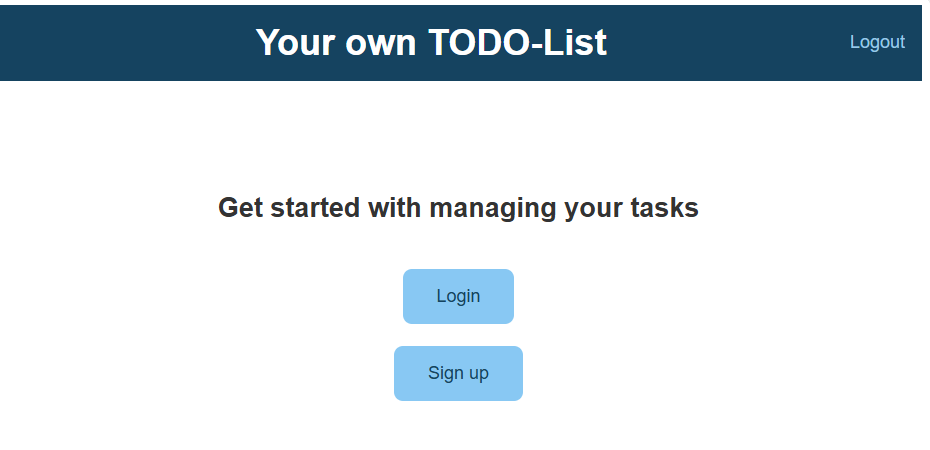
\includegraphics[clip,width=0.75\linewidth]{images/index.png}
		\caption[User Interface Design der Startseite]{User Interface Design der Startseite [Eigene Darstellung]}
		\label{UI_index}
	\end{figure}	
	
	\item \textbf{/LoginView}: Die Anmeldeseite siehe Abbildung \ref{UI_logIn}. Hier können Benutzer ihren Benutzernamen und ihr Passwort eingeben, um auf ihre persönlichen Aufgabenlisten zuzugreifen. Ein Link zur Registrierung ist ebenfalls vorhanden.
	
	\begin{figure}[h]
		\centering
		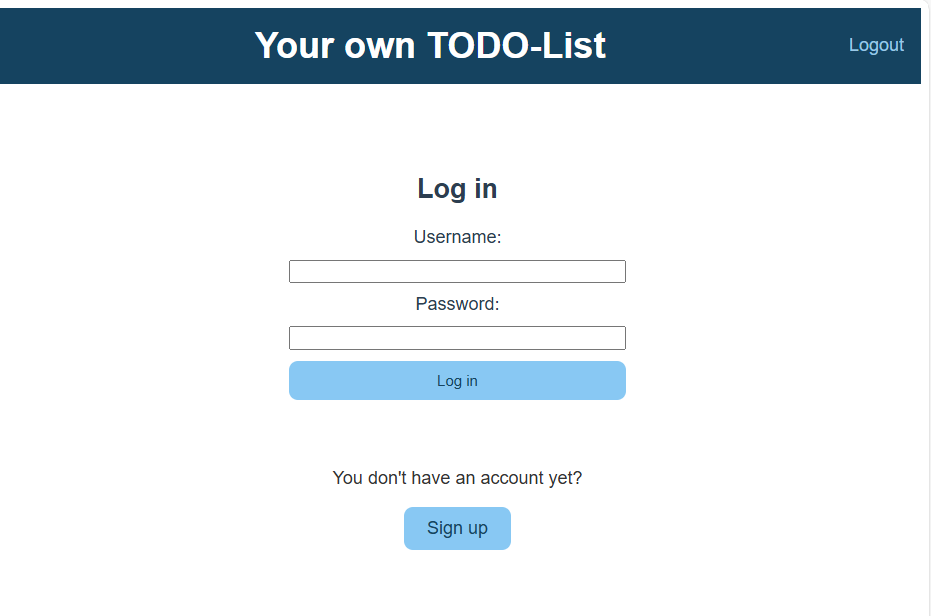
\includegraphics[clip,width=0.75\linewidth]{images/logIn.png}
		\caption[User Interface Design der Anmeldeseite]{User Interface Design der Anmeldeseite [Eigene Darstellung]}
		\label{UI_logIn}
	\end{figure}	
	
	\item \textbf{/RegisterView}: Die Registrierungsseite siehe Abbildung \ref{UI_signUp}. Neue Benutzer können hier ein Konto erstellen, indem sie ihren Benutzernamen, ihr Passwort und die Bestätigung des Passworts eingeben. Ein Link zur Anmeldung für bestehende Benutzer ist ebenfalls verfügbar.
	
	\begin{figure}[h]
		\centering
		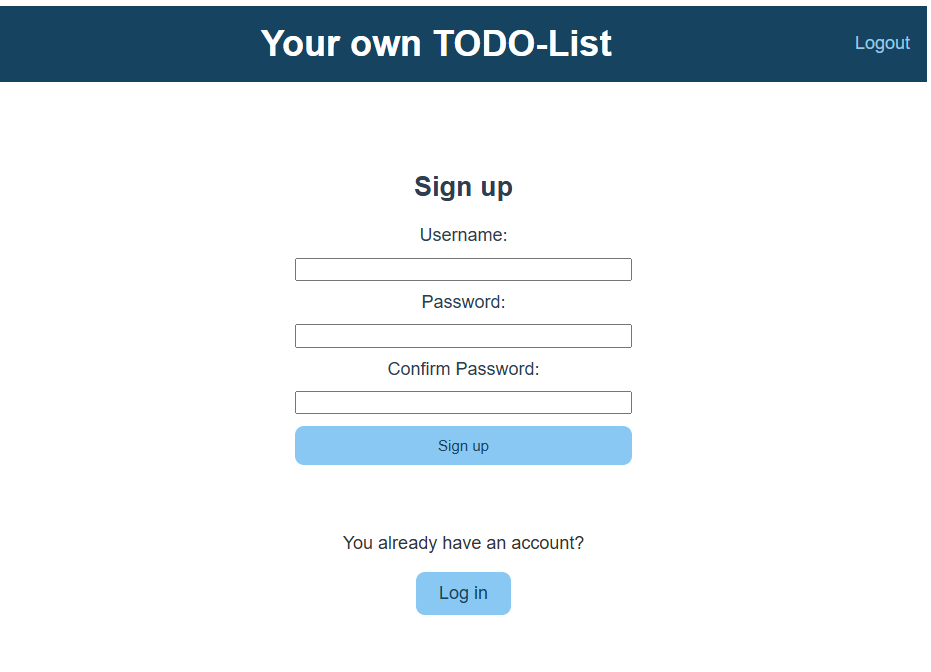
\includegraphics[clip,width=0.75\linewidth]{images/signUp.png}
		\caption[User Interface Design der Registrierungsseite]{User Interface Design der Registrierungsseite [Eigene Darstellung]}
		\label{UI_signUp}
	\end{figure}	
	
	\item \textbf{/HomeView}: Die Hauptseite nach der Anmeldung siehe Abbildung \ref{UI_home}. Diese Seite zeigt die Aufgabenliste des angemeldeten Benutzers. Benutzer können neue Aufgaben erstellen, vorhandene Aufgaben bearbeiten oder löschen.
	
	\begin{figure}[h]
		\centering
		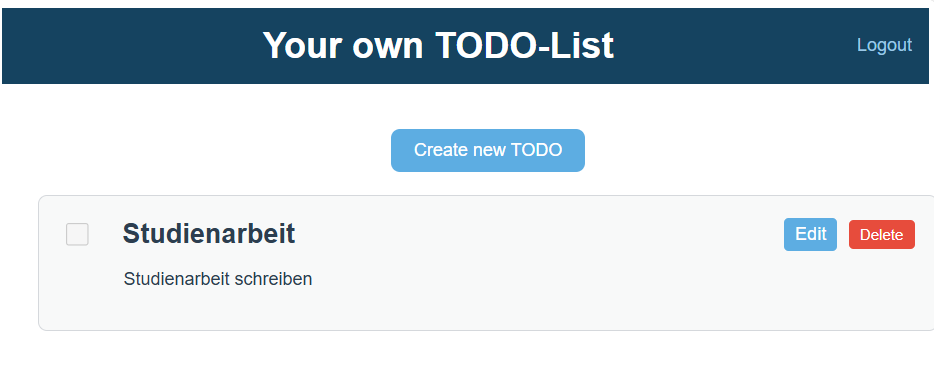
\includegraphics[clip,width=0.75\linewidth]{images/home.png}
		\caption[User Interface Design der Hauptseite]{User Interface Design der Hauptseite [Eigene Darstellung]}
		\label{UI_home}
	\end{figure}	
	
	\item \textbf{/NewTodoForm}: Diese Seite bietet ein Formular zum Erstellen einer neuen Todo siehe Abbildung \ref{UI_newTodo}.
	% TODO
	
	\begin{figure}[h]
		\centering
		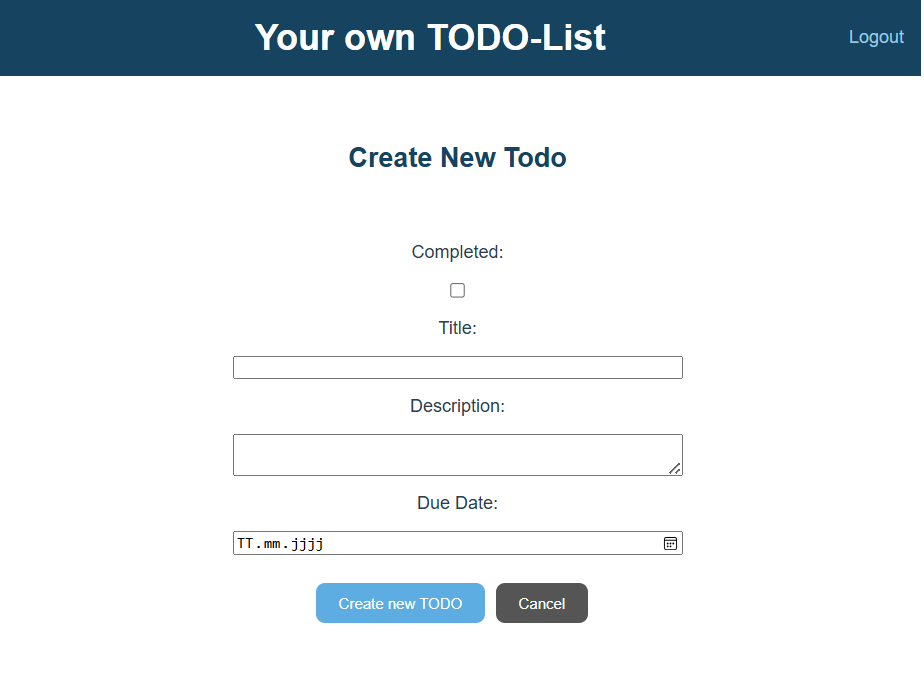
\includegraphics[clip,width=0.75\linewidth]{images/newTodo.png}
		\caption[User Interface Design der Ansicht zum Erstellen einer neuen Todo]{User Interface Design der Ansicht zum Erstellen einer neuen Todo [Eigene Darstellung]}
		\label{UI_newTodo}
	\end{figure}
	
	\item \textbf{/TodoDetailView}: Die Detailansicht einer spezifischen Todo siehe Abbildung \ref{UI_idTodo}. Diese Seite ermöglicht es Benutzern, die Details einer ausgewählten Todo zu bearbeiten.
	
	\begin{figure}[h]
		\centering
		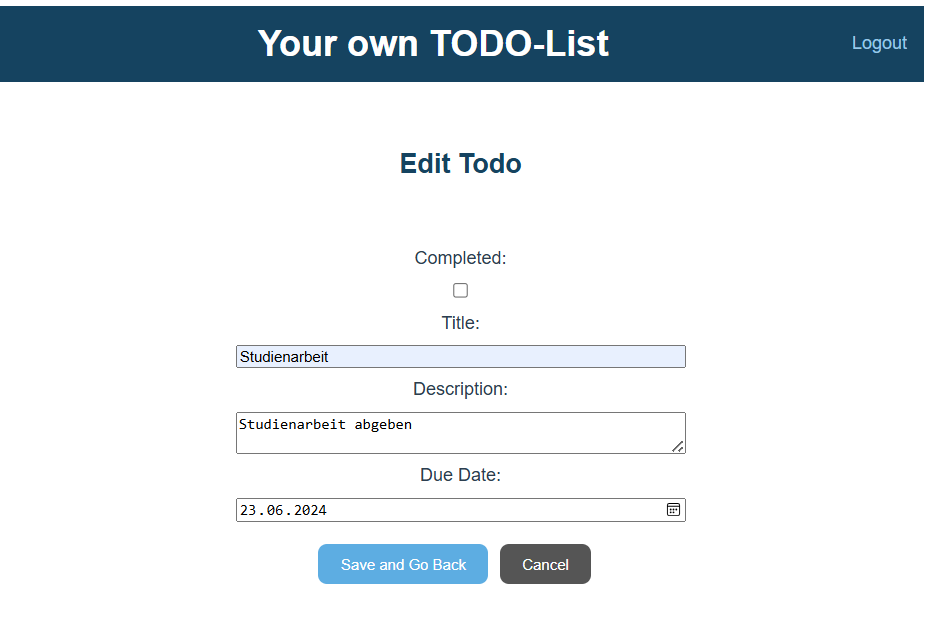
\includegraphics[clip,width=0.75\linewidth]{images/idTodo.png}
		\caption[User Interface Design der Detailansicht zum Bearbeiten]{User Interface Design der Detailansicht [Eigene Darstellung]}
		\label{UI_idTodo}
	\end{figure}	
	
\end{itemize}

Jede Seite hat ein konsistentes Layout mit einem zentralen Header. Der Header ist als eine Komponente in der \textbf{/HeaderBar} definiert. Er enthält das Logo "`Your own TODO-List"' und die Logout-Option, abhängig davon, ob der Benutzer angemeldet ist.

\subsection{Berücksichtigung von Usability-Prinzipien}

Das User Interface Design der Todo-App folgt mehreren grundlegenden Usability-Prinzipien nach Jakob Nielsen \cite{nielsen_10_nodate}, um sicherzustellen, dass die Anwendung einfach zu bedienen und effizient ist:

\begin{enumerate}
	\item \textbf{Sichtbarkeit des Systemstatus}: Die App hält den Benutzer stets über den aktuellen Status und die Ergebnisse ihrer Aktionen informiert. Beispielsweise werden Änderungen an Aufgaben sofort angezeigt und erfolgreiche Anmeldungen führen direkt zur Hauptseite mit der Aufgabenliste.
	\item \textbf{Übereinstimmung zwischen System und realer Welt}: Die Anwendung verwendet Begriffe und Konzepte, die den Benutzern vertraut sind. Schaltflächen und Symbole sind intuitiv und leicht verständlich, was die Bedienung erleichtert.
	\item \textbf{Benutzerkontrolle und Freiheit}: Benutzer können Aktionen rückgängig machen. Es gibt deutlich sichtbare Optionen zum Abbrechen von Aktionen, um Fehlaktionen leicht korrigieren zu können.
	\item \textbf{Konsistenz und Standards}: Das Layout und das Design der Benutzeroberfläche sind auf allen Seiten der Anwendung konsistent. Dies erleichtert den Benutzern das Verständnis und die Navigation durch die App.
	%\item \textbf{Fehlervermeidung}: Die Anwendung enthält Sicherheitsabfragen und Bestätigungsdialoge, um unbeabsichtigte Aktionen zu verhindern. Beispielsweise wird vor dem Löschen einer Aufgabe eine Bestätigung eingeholt.
	% TODO: mit rein nehmen, wenn es sicherheitsabfragen gibt
	\item \textbf{Wiedererkennung statt Erinnerung}: Die Benutzeroberfläche macht alle wichtigen Optionen und Funktionen sichtbar, damit Benutzer sie leicht wiedererkennen können, anstatt sich an sie erinnern zu müssen. Wichtige Elemente wie Schaltflächen und Eingabefelder sind prominent platziert und leicht zu finden. Der Einsatz von Farben und Schriftgrößen hilft, die Aufmerksamkeit der Benutzer auf wichtige Aktionen und Informationen zu lenken.
	%\item \textbf{Flexibilität und Effizienz der Nutzung}: 
	\item \textbf{Ästhetik und minimalistisches Design}: Das Design ist einfach und übersichtlich gehalten, um die Benutzerfreundlichkeit zu erhöhen. Unnötige Elemente wurden vermieden, um Ablenkungen zu minimieren und den Fokus auf die Hauptfunktionen der Anwendung zu legen.
	\item \textbf{Hilfe beim Erkennen, Diagnostizieren und Beheben von Fehlern}: Fehlernachrichten sind in einfacher Sprache verfasst und bieten klare Hinweise zur Problemlösung. Beispielsweise wird bei einer fehlerhaften Anmeldung eine verständliche Fehlermeldung angezeigt und mögliche Lösungen vorgeschlagen.
	% TODO: Fehlermeldungen und Lösungsmöglichkeiten
	%\item \textbf{Hilfe und Dokumentation}: Obwohl die App so gestaltet ist, dass sie intuitiv bedienbar ist, steht den Benutzern bei Bedarf eine leicht durchsuchbare Hilfedokumentation zur Verfügung. Diese enthält konkrete Anleitungen zur Durchführung von Aufgaben.
\end{enumerate}





\chapter{Backend-Implementierung unter Verwendung von TDD}

\section{Entwicklungsumgebung und Werkzeuge}

Die Entwicklung der Todo-App erfolgte in einer modernen Java-Entwicklungsumgebung, die auf dem Spring Boot Framework basiert. Die wichtigsten verwendeten Tools und Technologien sind:

\begin{itemize}
	\item \textbf{IDE}: IntelliJ IDEA wurde als Integrated Development Environment (IDE) verwendet, da es umfangreiche Unterstützung für Java und das Spring Framework bietet, einschließlich leistungsstarker Debugging- und Refactoring-Tools \cite{noauthor_intellij_nodate}. 
	\item \textbf{Build-Tool}: Maven wurde für das Build-Management und die Abhängigkeitsverwaltung eingesetzt. Es ermöglicht die einfache Verwaltung von Bibliotheken und Plugins sowie die Konfiguration von Build-Prozessen \cite{noauthor_maven_nodate}. 
	\item \textbf{Versionierung}: GitHub wurde für die Quellcodeverwaltung und Versionskontrolle verwendet. GitHub ermöglichte zudem die Zusammenarbeit und den Austausch von Code \cite{noauthor_build_2024}.
	\item \textbf{Test-Frameworks}: JUnit 5 und Spring Boot Test wurden für die Implementierung und Ausführung von Unit- und Integrationstests verwendet. Mockito diente zur Erstellung von Mock-Objekten für die Isolierung von Testfällen.
	\item \textbf{Datenbank}: MySQL wurde als relationale Datenbank verwendet. Für die Tests wurde eine MySQL-Testdatenbank konfiguriert, um schnelle und isolierte Testausführungen zu ermöglichen. Für die Entwicklungsumgebung wurde XAMPP verwendet, das eine einfache Möglichkeit bietet, einen lokalen Webserver mit MySQL-Datenbank zu betreiben \cite{noauthor_xampp_nodate}.

\end{itemize}

\section{Implementierungsschritte}

Die Implementierung am Beispiel der Benutzerregistrierung in der Todo-App folgte nach dem klassischen TDD-Zyklus: \textbf{Red-Green-Refactor}.

\begin{enumerate}
	\item \textbf{Red Phase}: Zunächst wurde ein fehlgeschlagener Test (Red) geschrieben, der die Registrierung eines neuen Benutzers beschreibt, ohne dass die Implementierung vorhanden war.
	
	Beispiel: Ein Test für die Registrierung eines neuen Benutzers über den UserController.
	\begin{lstlisting}[language=Java]
		@Test
		public void testRegisterUser_success() throws Exception {
			UserRegistrationRequest request = new UserRegistrationRequest();
			request.setUsername("integrationtestuser");
			request.setPassword("password");
			request.setConfirmPassword("password");
			
			ResultActions result = mockMvc.perform(post("/register")
			.contentType(MediaType.APPLICATION_JSON)
			.content(objectMapper.writeValueAsString(request)));
			
			result.andExpect(status().isOk());
		}
	\end{lstlisting}
	
	\item \textbf{Green Phase}: Anschließend wurde der minimal notwendige Code geschrieben, um den Test erfolgreich zu bestehen (Green). In diesem Schritt wird nur so viel implementiert, dass der Testfall erfüllt wird.
	
	Beispiel: Die grundlegende Implementierung des registerUser-Endpunkts im UserController.
	
	\begin{lstlisting}[language=Java]
		@PostMapping("/register")
		public ResponseEntity<?> registerUser(@RequestBody UserRegistrationRequest request) {
			User user = new User();
			user.setUsername(request.getUsername());
			user.setPassword(passwordEncoder.encode(request.getPassword()));
			
			return ResponseEntity.ok(user);
		}
	\end{lstlisting}
	
	\item \textbf{Refactor Phase}: Nach dem erfolgreichen Bestehen des Tests wurde der Code optimiert und verbessert, ohne die Funktionalität zu ändern. Dabei wurde auf Sauberkeit, Lesbarkeit und Wartbarkeit des Codes geachtet.
	
	Beispiel: Die vollständige Implementierung des registerUser-Endpunktes im UserController zeigt, dass ein Refactoring erfolgte, nachdem die Implementierung zum erfolgreichen Ausführen von Test, wie zum Beispiel des Testens der Fehlerbehandlung von bereits existierenden Benutzernamen, hinzugefügt wurde.
	
	\begin{lstlisting}[language=Java]
		@PostMapping("/register")
		public ResponseEntity<?> registerUser(@Valid @RequestBody UserRegistrationRequest request, BindingResult result) {
			// Check if username already exists
			if (userService.existsByUsername(request.getUsername())) {
				return ResponseEntity.status(HttpStatus.CONFLICT).body("Username already exists");
			}
			
			// Check if password and confirmation match
			if (!request.getPassword().equals(request.getConfirmPassword())) {
				
				return ResponseEntity.status(HttpStatus.CONFLICT).body("Password and confirm password do not match");
			}
			
			// Check for validation results
			if (result.hasErrors()) {
				
				return ResponseEntity.status(HttpStatus.BAD_REQUEST).body("Validation error: " + result.getAllErrors());
			}
			
			// Register user
			try {
				User user = authenticationService.register(request);
				return ResponseEntity.ok(user);
			} catch (Exception e) {
				return ResponseEntity.status(HttpStatus.INTERNAL_SERVER_ERROR).body("Error registering user");
			}
		}
	\end{lstlisting}
	
\end{enumerate}

Die Anwendung des TDD-Zyklus unterstützt eine stabile Implementierung und kann zu einem fehlerarmen Code führen.

\section{Beispieltests und Testfälle}

\section{Unit-Tests}

Unit-Tests wurden verwendet, um einzelne Komponenten isoliert zu testen. 

Ein Beispiel ist der Test der \texttt{UserController}-Klasse, um sicherzustellen, dass eine Registrierung eines Benutzers erfolgreich verläuft.

\begin{lstlisting}[language=Java]
	@Test
	public void testRegisterUserPasswordMismatch() {
		UserRegistrationRequest request = new UserRegistrationRequest("testuser", "password1", "password2");
		
		BindingResult result = mock(BindingResult.class);
		ResponseEntity<?> response = userController.registerUser(request, result);
		
		assertEquals(HttpStatus.CONFLICT, response.getStatusCode());
		assertEquals("Password and confirm password do not match", response.getBody());
	}
\end{lstlisting}

\section{Integrationstests}

Integrationstests wurden durchgeführt, um das Zusammenspiel verschiedener Komponenten zu überprüfen. 

Ein Beispiel ist der Integrationstest für die Benutzerregistrierung über den \texttt{UserController}.

\begin{lstlisting}[language=Java]
	
	@Test
	public void testRegisterUserSuccess() throws Exception {
		UserRegistrationRequest request = new UserRegistrationRequest();
		request.setUsername("integrationtestuser");
		request.setPassword("password");
		request.setConfirmPassword("password");
		
		ResultActions result = mockMvc.perform(post("/register")
		.contentType(MediaType.APPLICATION_JSON)
		.content(objectMapper.writeValueAsString(request)));
		
		result.andExpect(status().isOk());
	}
\end{lstlisting}


\section{Akzeptanztests}

Akzeptanztests wurden verwendet, um sicherzustellen, dass die Anwendung den Anforderungen der Benutzer entspricht. Diese Tests wurden aus der Sicht des Endbenutzers geschrieben und überprüfen die Funktionalität der gesamten Anwendung.

Ein Beispiel ist der Akzeptanztest für die Benutzerregistrierung über die REST-Schnittstelle.


\begin{lstlisting}[language=Java]

	@Test
	public void testRegisterUser() {
		String url = "http://localhost:" + port + "/register";
		UserRegistrationRequest request = new UserRegistrationRequest("testuser", "password", "password");
		
		HttpHeaders headers = new HttpHeaders();
		HttpEntity<UserRegistrationRequest> entity = new HttpEntity<>(request, headers);
		
		// Send HTTP POST request
		ResponseEntity<String> response = restTemplate.exchange(url, HttpMethod.POST, entity, String.class);
		
		// Check if the response status code is 409 (CONFLICT)
		assertEquals(HttpStatus.CONFLICT, response.getStatusCode());
	}
	
\end{lstlisting}

Diese strukturierte Vorgehensweise durch TDD unterstützt eine robuste und fehlerarme Implementierung der Todo-Liste.


\chapter{Frontend Entwicklung}
\section{Projektanforderung an Frontend-Entwicklung}

Das Projekt stellt vielfältige  Anforderungen an die Entwicklung des Frontends:

\begin{itemize}
	\item \textbf{Einfachheit und Flexibilität}:  Vue.js bietet eine sanfte Lernkurve und ist flexibel einsetzbar, was es ideal für verschiedene Projektanforderungen macht \cite{noauthor_vuejs_nodate}.
	
	\item \textbf{Einfache Integrität}: Vue.js ermöglicht eine einfache Integration in bestehende Projekte und Technologiestacks \cite{noauthor_vuejs_nodate}.
	
	\item \textbf{Reaktive Datenbindung}: Durch die reaktive Datenbindung können Änderungen automatisch auf der Benutzeroberfläche reflektiert werden, was die Entwicklung dynamischer Anwendungen erleichtert \cite{noauthor_vuejs_nodate}.
	
	\item \textbf{Komponentenbasierte Architektur}: Die komponentenbasierte Architektur fördert die Wiederverwendbarkeit und Wartbarkeit des Codes, indem sie die Trennung von Logik und Darstellung erleichtert \cite{noauthor_vuejs_nodate}.
	
	\item \textbf{Leistungsfähigkeit}: Vue.js bietet eine hohe Leistung und Effizienz bei der Erstellung von Benutzeroberflächen \cite{noauthor_vuejs_nodate}.
	
	\item \textbf{Große Community und gute Dokumentation}: Eine aktive Community und umfassende Dokumentation erleichtern die Lösung von Problemen und den Zugriff auf Ressourcen \cite{noauthor_vuejs_nodate}.
\end{itemize}

Die Wahl von Vue.js als Framework erfüllt diese Anforderungen und rechtfertigt daher die Entscheidung für seine Verwendung im Projekt.


\section{Technologiestack}

Das Frontend verwendet folgende Technologien und Frameworks:

\begin{itemize}
	\item \textbf{Vue.js (Version 3.2.13)}: Haupt-Framework für die Erstellung der Benutzeroberfläche.
	\item \textbf{Vue Router (Version 4.4.0)}:  Routing-Library für die Navigation innerhalb der Anwendung.
	\item \textbf{Vuex (Version 4.1.0}: State-Management-Bibliothek für die zentralisierte Speicherung von Daten.
\end{itemize}

Das Projekt wurde mit Hilfe des Vue CLI (Command Line Interface) initialisiert, um eine standardisierte Projektstruktur und die notwendigen Abhängigkeiten bereitzustellen. Nach der Erstellung des Projekts wurden die zusätzliche Bibliotheken \texttt{axios} für HTTP-Anfragen und \texttt{vue-router} für die Navigation installiert.


\section{Projektstruktur}
Die Projektstruktur wurde so gestaltet, dass sie eine klare Trennung der einzelnen Komponenten und Funktionalitäten ermöglicht. Die Verzeichnisstruktur ist wie folgt:

\begin{itemize}
	\item \textbf{/src}: Hauptverzeichnis für den Quellcode.
	\item \textbf{/src/components}: Enthält wiederverwendbare Vue-Komponenten.
	\item \textbf{/src/components/HeaderBar.vue}: Die Kopfzeile der Anwendung, die das Logo und die Logout-Option enthält, abhängig davon, ob der Benutzer angemeldet ist.
	\item \textbf{/src/views}: Enthält die Hauptansichten der Anwendung.
	\item \textbf{/src/views/IndexView.vue}: Die Startseite der Anwendung, die Optionen zum Anmelden und Registrieren bereitstellt.
	\item \textbf{/src/views/LoginView.vue}: Das Anmeldeformular, das Benutzername und Passwort für die Authentifizierung erfordert.
	\item \textbf{/src/views/RegisterView.vue}: Das Registrierungsformular, das Benutzer zur Erstellung eines Kontos ermöglicht.%TODO Konto oder Account
	\item \textbf{/src/views/HomeView.vue}: Die Hauptansicht nach der Anmeldung, die eine Liste von Todos anzeigt.
	\item \textbf{/src/views/NewTodoForm.vue}: Ein Formular zur Erstellung neuer Todos.
	\item \textbf{/src/views/TodoDetailView.vue}: Ansicht zum Bearbeiten eines bestimmten Todos.
	\item \textbf{/src/router.js}: Konfiguration der Vue Router-Instanz.
	\item \textbf{/src/store.js}: Vuex Store-Konfiguration für das State-Management.
	\item \textbf{/src/App.vue}: Wurzelkomponente der Anwendung.
	\item \textbf{/src/main.js}: Einstiegspunkt, wo die Vue-Instanz erstellt und konfiguriert wird.

\end{itemize}

\section{Routing}
Der Router wurde in der Datei \texttt{src/router.js} konfiguriert. Die Konfiguration umfasst die Definition der verschiedenen Routen, die jeweils einer spezifischen Komponente zugeordnet sind. Dies ermöglicht eine einfache Navigation zwischen den verschiedenen Ansichten der Anwendung.
	
\section{Authentifizierung und Autorisierung}
Die Webanwendung verwendet JSON Web Tokens (JWT) zur Authentifizierung von Benutzern. Nach erfolgreicher Anmeldung wird ein Token im Local Storage gespeichert und für alle folgenden Anfragen an den Server verwendet. Die Authentifizierung wird durch Vue Router Navigation Guards implementiert, um sicherzustellen, dass nur authentifizierte Benutzer auf geschützte Routen zugreifen können.

\section {HTTP-Anfragen}
HTTP-Anfragen werden mit Axios durchgeführt, um mit dem Backend-Server zu kommunizieren. Diese Anfragen werden in den Vue-Komponenten ausgeführt, um Daten zu laden, zu speichern oder zu aktualisieren.
Für jede wird der JWT-Token automatisch zum Header hinzugefügt, um sicherzustellen, dass der Server die Anfrage autorisiert.

\section{State Management}
Vuex wird verwendet, um den globalen Zustand der Anwendung zu verwalten. Es speichert den Anmeldestatus und den JWT-Token des Benutzers und bietet zentralisierten Zugriff auf diese Daten. Die State-Management-Logik wurde in der Datei \texttt{src/store.js} definiert.

\section{Styling}
Das Styling erfolgt hauptsächlich mit CSS innerhalb der einzelnen Vue-Komponenten. Das Scoped Styling von Vue.js sorgt dafür, dass die Styles nur auf die jeweilige Komponente angewendet werden.





\chapter{Deployment}

Um die Todo-Liste Webanwendung bereitzustellen und zu starten, sind mehrere Schritte erforderlich, einschließlich der Einrichtung der Datenbank und der Ausführung der Anwendung sowohl für das Frontend als auch das Backend.

\section{Datenbank einrichten}

Zunächst muss die MySQL-Datenbank eingerichtet werden, um die Daten der Todo-Liste speichern zu können. Für die Entwicklungsumgebung wurde XAMPP verwendet, das eine einfache Möglichkeit bietet, einen lokalen Webserver mit MySQL-Datenbank zu betreiben. Für die Konfiguration können die folgenden Informationen aus der application.properties verwendet werden:

\begin{lstlisting}
spring.datasource.url=jdbc:mysql://localhost:3306/todoappdb
spring.datasource.username=springuser
spring.datasource.password=123456
spring.datasource.driver-class-name=com.mysql.cj.jdbc.Driver
spring.jpa.hibernate.ddl-auto=update
spring.jpa.show-sql=true
spring.jpa.properties.hibernate.dialect=org.hibernate.dialect.MySQL8Dialect
\end{lstlisting}

das notwendige Datenbankdesign, kann aus dem Kapitel 3.2.3 Datenbankdesign entnommen werden.


\section{Backend starten}
Das Backend der Todo-Liste Webanwendung ist mit Spring Boot implementiert. Hier sind die Schritte zum Starten des Backends:

\begin{enumerate}
	\item \textbf{Projekt herunterladen und öffnen:} Das Projekt muss zunächst von dem Versionskontrollsystem Github geruntergeladen werden und anschließend in einer bevorzugten IDE geöffnet werden \cite{noauthor_philippabeletdd--java_nodate}. 	%Verweis auf sein Projekt
	\item \textbf{Konfigurieren der Datenbankverbindung:} Die Datenbankeinstellungen in der Datei "`src/main/resources/application.properties"' müssen so angepasst sein, dass Zugriff auf die zuvor erstellte Datenbank ermöglicht werden kann.
	\item \textbf{Starten der Backends:} Die Spring Boot-Anwendung kann mittels dem Aufrufen der "`main"'-Methode in der Hauptklasse ("`TodoApplication"') gestartet werden.
\end{enumerate}

\section{Frontend starten}
Das Frontend der Todo-Liste Webanwendung basiert auf Vue.js. Hier sind die Schritte zum Starten des Frontends:

\begin{enumerate}
	\item \textbf{Projekt herunterladen und öffnen:} Das Projekt muss zunächst von dem Versionskontrollsystem Github geruntergeladen werden und anschließend in einer bevorzugten IDE geöffnet werden \cite{noauthor_philippabeletdd--java_nodate}. .
	\item \textbf{Installieren der Abhängigkeiten:} Mittels einer Befehlszeile kann zum Verzeichnis des Frontend-Projekts navigiert werden. Durch den Befehl "`npm install"' werden alle Abhängigkeiten installiert, die in der "`package.json"'-Datei aufgeführt sind.
	\item \textbf{Starten der Frontends:} Nachdem alle Abhängigkeiten installiert wurden, kann das Frontend mit dem Befehl "`npm run serve"' gestartet werden.
\end{enumerate}
	
\section{Zugriff auf Todo-Liste Webanwendung}
Nachdem sowohl das Backend als auch das Frontend gestartet wurde, kann auf die Todo-Liste Webanwendung zugegriffen werden. Hierfür muss ein Webbrowser geöffnet und zu der URL "`localhost:8081"' navigiert werden. Es erscheint die Startseite der Todo-Liste, in der sich registriert oder angemeldet werden kann.


\chapter{Fazit}
Diese Studienarbeit zielt darauf ab, eine intuitive Benutzererfahrung zu bieten, die es Benutzern ermöglicht, Todos zu erstellen, zu bearbeiten und zu löschen, sowie zusätzliche Details wie Beschreibungen und Fälligkeitsdaten hinzuzufügen.

Die entwickelte Todo-Liste besteht aus zwei Hauptkomponenten: dem Frontend, das auf Vue.js basiert und die Benutzeroberfläche bereitstellt, und dem Backend, das auf Spring Boot aufbaut und die Datenverarbeitung und -speicherung übernimmt. Die Integration mit einer MySQL-Datenbank bietet eine robuste Grundlage für die Speicherung von Benutzerdaten und Todos.

Trotz der erfolgreichen Implementierung der grundlegenden Funktionen der Todo-Liste gibt es noch einige Herausforderungen und unvollständige Aspekte, die erwähnt werden müssen. Ein Benutzer kann sich erfolgreich registrieren und anmelden, jedoch sind die Funktionen zur sicheren Abmeldung und zur Bearbeitung von Todos nicht vollständig implementiert. Dies führt zu Bedenken hinsichtlich der Privatsphäre und der Benutzerfreundlichkeit der Anwendung.

Die Gründe für diese unvollständigen Funktionen sind vielschichtig. Der begrenzte Erfahrungsschatz des Entwicklers mit den verwendeten Technologien sowie unzureichendes Zeitmanagement haben dazu geführt, dass der ursprüngliche Zeitplan nicht eingehalten werden konnte. Zudem wurde der Zyklus des Test-Driven Developments (TDD) nicht konsequent durchgeführt vor allem im Hinblick des Refactoring, was zu nicht bestandenen Tests und vermutlich fehlerhaftem Code führte. Diese Probleme haben sich direkt auf die Funktionalität der Anwendung ausgewirkt, insbesondere auf Bereiche wie das sichere Ausloggen und die Bearbeitung von Todos.

Für zukünftige Weiterentwicklungen und Verbesserungen der Todo-Liste Webanwendung ist es entscheidend, diese Herausforderungen zu adressieren. Ein verstärkter Fokus auf Schulung und Weiterbildung in den verwendeten Technologien sowie eine verbesserte Projektplanung und -überwachung können helfen, ähnliche Probleme in zukünftigen Entwicklungsprojekten zu vermeiden. Darüber hinaus sollte die Implementierung von Best Practices im Bereich Softwareentwicklung, einschließlich eines strengeren TDD-Ansatzes und einer umfassenden Testabdeckung, Priorität haben, um die Qualität und Zuverlässigkeit der Anwendung sicherzustellen.

Insgesamt bietet diese Studienarbeit einen detaillierten Einblick in die Architektur, Implementierung und die Lessons Learned bei der Entwicklung der Todo-Liste Webanwendung. Trotz der identifizierten Herausforderungen legt sie den Grundstein für künftige Verbesserungen und Erweiterungen dieser digitalen Werkzeuge zur Aufgabenverwaltung.

\backmatter
\sloppy
\printbibliography
\addcontentsline{toc}{chapter}{Literaturverzeichnis}

\end{document}